\documentclass[usenames,dvipsnames,tikz]{standalone}
%\usepackage{amsmath,amssymb}
%\usepackage{xcolor}
\colorlet{tBlue}{RoyalBlue!35!Cerulean}
\colorlet{tRed}{Red}
%\usepackage{tikz}
%\usepackage{standalone}
\begin{document}
	
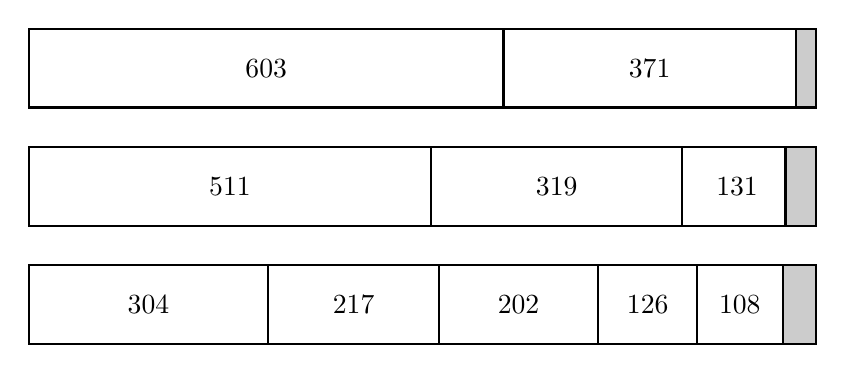
\begin{tikzpicture}
%\draw [help lines] (-1,-2) grid (11,5);
% 1=0.1, 2=0.15, 3=0.2, 4=0.25, 5=0.3
% 6 (3-27), 5 (8-42), 4 (33-65), 4 (16-22), 3 (13-28), 3 (11-40), 2 (35-50), 1 (15-30), 1 (14-38), 1 (4-57).


% BPP
\draw [thick] (0,0) rectangle (10,1); %bottom row
\draw [thick] (0,1.5) rectangle (10,2.5); %middle row
\draw [thick] (0,3) rectangle (10,4); %top row
 
% Bottom row, 304, 217, 202, 126, 108 (13-28 X 11-40, 35-50 X 14-38 X 4-47)
\draw [thick] (3.04,0) -- (3.04,1);
\draw [thick] (5.21,0) -- (5.21,1);
\draw [thick] (7.23,0) -- (7.23,1);
\draw [thick] (8.49,0) -- (8.49,1);
\draw [thick, fill=black!20!white] (9.58,0) rectangle (10,1);

\node at (1.52, 0.5) {$304$};
\node at (4.125, 0.5) {$217$};
\node at (6.22, 0.5) {$202$};
\node at (7.86, 0.5) {$126$};
\node at (9.03, 0.5) {$108$};

% Middle row, 511, 335, 131 (8-42 X 16-22 X 15-30)
\draw [thick] (5.11,1.5) -- (5.11,2.5);
\draw [thick] (8.3,1.5) -- (8.3,2.5);
\draw [thick, fill=black!20!white] (9.61,1.5) rectangle (10,2.5);

\node at (2.555, 2) {$511$};
\node at (6.705, 2) {$319$};
\node at (8.995, 2) {$131$};

% Top row, 603, 382 (3-27 X 33-65)
\draw [thick] (6.03,3) -- (6.03,4);
\draw [thick, fill=black!20!white] (9.74,3) rectangle (10,4);

\node at (3.015, 3.5) {$603$};
\node at (7.885, 3.5) {$371$};

%--------------------------



\end{tikzpicture}

\end{document}